\documentclass{article}
\usepackage[utf8]{inputenc}
\usepackage[margin=1in]{geometry}

\title{CLASS - Homework NUMBER}
\author{Victor Zhang}
\date{JANUARY 1, 2000}

\usepackage[utf8]{inputenc}
\usepackage{amsmath}
\usepackage{amsfonts}
\usepackage{natbib}
\usepackage{graphicx}
% \usepackage{changepage}
\usepackage{amssymb}
\usepackage{xfrac}
% \usepackage{bm}
% \usepackage{empheq}
\usepackage{tikz}
\usepackage{pgfplots}
\usepackage{tikz-3dplot}

\newcommand{\contra}{\raisebox{\depth}{\#}}

\newenvironment{myindentpar}[1]
  {\begin{list}{}
          {\setlength{\leftmargin}{#1}}
          \item[]
  }
  {\end{list}}

\pagestyle{empty}

\begin{document}

\maketitle
% \begin{center}
% {\huge Econ 482 \hspace{0.5cm} HW 3}\
% {\Large \textbf{Victor Zhang}}\
% {\Large February 18, 2020}
% \end{center}

\section{}
Hello hello
\begin{figure}
\centering
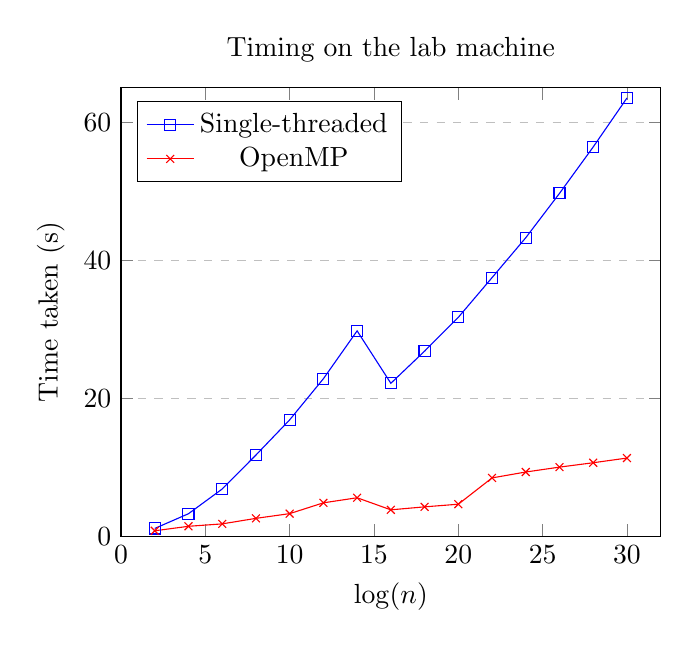
\begin{tikzpicture}
\begin{axis}[
    title={Timing on the lab machine},
    xlabel={$\log(n)$},
    ylabel={Time taken (s)},
    xmin=0, xmax=32,
    ymin=0, ymax=65,
    % xtick={0.0,0.2,0.4,0.6,0.8,1.0},
    % ytick={0.0,0.2,0.4,0.6,0.8,1.0},
    legend pos=north west,
    ymajorgrids=true,
    grid style=dashed,
]
\addplot[
    color=blue,
    mark=square,
    ]
    coordinates {
    (2,1.12144)(4,3.25651)(6,6.8407)(8,11.7633)(10,16.8647)(12,22.8305)(14,29.7678)(16,22.1659)(18,26.8288)(20,31.7287)(22,37.4847)(24,43.2715)(26,49.7034)(28,56.435)(30,63.5267)
    };
    \addlegendentry{Single-threaded}
\addplot[
    color=red,
    mark=x,
    ]
    coordinates {
    (2,0.78364)(4,1.43273)(6,1.78363)(8,2.58572)(10,3.26882)(12,4.83626)(14,5.57104)(16,3.82041)(18,4.25249)(20,4.6349)(22,8.44789)(24,9.30462)(26,10.0135)(28,10.6476)(30,11.3276)
    };
    \addlegendentry{OpenMP} 
        
\end{axis}
\end{tikzpicture}
\caption{Running on a 20-core machine}
\end{figure}

\end{document}

% List of tex snippets:
%   - tex-header (this)
%   - R      --> \mathbb{R}
%   - Z      --> \mathbb{Z}
%   - B      --> \mathcal{B}
%   - E      --> \mathcal{E}
%   - M      --> \mathcal{M}
%   - m      --> \mathfrak{m}({#1})
%   - normlp --> \norm{{#1}}_{L^{{#2}}}
